%%%%%%%%%%%%%%%%%%%%%%%%%%%%%%%%%%%%%%%%%%%%%%%%%%%%%%%%%%%%%%%%%%
\section{Análisis de los datasets disponibles}
\label{sec:sustdata}

En ámbitos como el Procesado de Lenguaje Natural (del inglés \gls{nlp}) o el reconocimiento facial, la disponibilidad de numerosas fuentes de datos ha sido imprescindible para acelerar el desarrollo de técnicas de minería de datos y de aprendizaje automático (\gls{ml}).

\vspace{3mm}

A diferencia de estos campos, el contexto energético experimenta un menor grado de disponiblidad de datasets. La protección de la privacidad de los usuarios en el proceso de medición y análisis de su comportamiento energético supone que exista un menor número de datasets públicos enfocados a implementaciones reales. No obstante, la búsqueda de la optimización de la distribución energética y de la reducción del consumo de los usuarios, aparte de otras motivaciones ambientales, ha instado en los últimos años a múltiples ingenieros y científicos a lo largo del mundo a crear datasets públicos enfocados a la investigación (ver Tabla \ref{tab:datasets}). 

\vspace{3mm}

En este contexto han cobrado gran importancia las técnicas de Monitorización de Cargas no Intrusiva (del inglés \gls{nilm}). Como se ha introducido en la Sección \ref{sec:ioe}, cada vez se produce una mayor integración de las tecnologías de \gls{ioe} en el ámbito de las \gls{sg}s para obtener una mayor monitorización del comportamiento energético en los hogares. Es por ello que el fin principal de las técnicas de \gls{nilm} reside en establecer una desagregación energética para poder estimar de una forma precisa el consumo individual de cada uno de los dispositivos y electrodomésticos que hay en una vivienda. Para ello, se instalan medidores en cada circuito y después, se analizan, tanto a nivel interno como a nivel externo de la vivienda, los cambios de los parámetros eléctricos en cada instante temporal.~\cite{nilm} \cite{greend}

\vspace{3mm}

Teniendo esto en cuenta, se puede expresar que las técnicas de \gls{nilm} se caracterizan por su bajo coste y por su facilidad y flexibilidad de despliegue. No obstante, el proceso de medición y recolección de datos puede llegar a requerir mucho tiempo y esfuerzo. Por ello, en el contexto de la investigación es importante que los datos tengan una disponibilidad pública para progresar en el desarrollo de técnicas de minería de datos y de aprendizaje automático en el ámbito energético. 

\vspace{3mm}

En la Tabla \ref{tab:datasets} se exponen los múltiples datasets residenciales que han sido estudiados en esta fase de diseño, junto con información relativa a la implementación real sobre la que se ha basado cada uno de ellos, como es la ubicación de la misma, el número de viviendas total, el lapso temporal que comprende el despliegue, la frecuencia de las muestras tomadas y los parámetros eléctricos medidos. En virtud de las motivaciones y objetivos del presente \gls{tfm}, es importante tener en cuenta ciertos requisitos para evaluar los conjuntos de datos disponibles y seleccionar el más apropiado:

\vspace{1mm}

\begin{itemize}
    \item Cantidad: En primera instancia, es imprescindible revisar la cantidad de datos que aporta cada conjunto. En otros términos, para llevar a cabo un análisis estadístico del comportamiento energético de una ubicación se requiere partir de un conjunto de datos que agrupe las mediciones de un gran número de edificios residenciales. Adicionalmente, este análisis debe comprender extensos períodos temporales de medición para visualizar de forma correcta el comportamiento de los usuarios y predecir patrones de consumo a lo largo del tiempo.
    \item Calidad: Se debe evaluar la calidad de los datos recogidos, la cual responde en parte con la resolución de las medidas que se toman. Como se puede observar en la Tabla \ref{tab:datasets}, algunos datasets como \textit{REDD} y \textit{BLUED} se centran en monitorizar los edificios residenciales a una frecuencia de muestreo alta. En el contexto de las tecnologías de \gls{nilm}, esto aporta una vista más representativa del comportamiento energético a nivel interno en una vivienda y permite una desagregación energética más precisa. Por lo tanto, cuanto mayor sea la frecuencia de adquisición de medidas, mayor será la resolucion de los datos. 
    
    \clearpage

    \item Ubicación: En términos de la ubicación de la implementación real sobre la que se han adquirido las mediciones, es de importancia conocer a la hora de analizar los datos las diferencias de voltaje que se manejan en cada país. Por ejemplo, en el caso de datasets como \textit{BLUED} o \textit{Smart*}, los cuales provienen de ciudades de Estados Unidos, trabajarán a tensiones menores de 120V, mientras que otros como \textit{ECO} o \textit{GREEND}, cuyos datos se han adquirido en países europeos, lo harán con tensiones de hasta 230V. \cite{greend} \cite{powercons}
    \item Parametrización: Por lo general, un dataset dedicado a las tecnologías de \gls{nilm} estará constituido por una colección de muestras de voltaje (V), corriente (I) y potencia activa (P), reactiva (Q) y aparente (S). Cada una de estas muestras vendrá asociada a una marca de tiempo y a un identificador que haga referencia a la vivienda o medidores a los que corresponde. Adicionalmente, algunos de los datasets que se exponen en la Tabla \ref{tab:datasets}, como son \textit{HUE} o \textit{SustDataED}, también incluyen información relativa a parámetros ambientales. Esto, sobre todo en el contexto de las \gls{sg}s, proporciona información fundamental sobre el impacto de las condiciones climáticas en el comportamiento de los usuarios.
    \item Generación fotovoltaica: Considerando el contexto de \gls{sg}s en el que se engloba este \gls{tfm}, es de vital importancia seleccionar un conjunto de datos que aporte información relativa a la generación de energía a través de fuentes renovables, como ocurre en el caso de \textit{Smart*} o \textit{SustDataED}. En relación con esto, se expondrá en la Sección \ref{sec:global} el estudio de una plataforma específica dedicada a la adquisición de datos de generación energética.
\end{itemize}

\begin{sidewaystable}
    \centering 
    \begin{tabularx}{\textheight}{|X|X|X|X|X|X|}
        \hline
        \rowcolor[HTML]{EFEFEF} 
        Nombre & Localización & Nº de residencias & Período de medición (días) & Resolución de medición & Parámetros \\ \hline
        \textit{AMPds2} \cite{ampds2} & Vancouver (Canadá) & 1 & 730 & 1min &  I, V, P, S, F, pf \\ \hline
        \textit{BLUED} \cite{blued} & Pittsburg (Estados Unidos) & 1 & 8 & 12KHz &  I, V, eventos de switch \\ \hline
        \textit{ECO} \cite{eco} & Thun (Suiza) & 6 & 244 & 1Hz & P \\ \hline
        \textit{GREEND} \cite{greend} & Italia y Austria & 9 & 310 & 1Hz & P \\ \hline
        \textit{HUE} \cite{hue} & British Columbia, Canada & 28 & 60 & 1Hz & P \\ \hline
        \textit{iAWE} \cite{iawe} & Nueva Delhi (La India) & 1 & 73 & 1Hz & V, I, P, S \\ \hline
        \textit{REDD} \cite{redd} & Boston (Estados Unidos) & 6 & 119 & 15KHz & I, V, P \\ \hline
        \textit{Smart*} \cite{smart*} & Massachussets (Estados Unidos) & 3 & 90 & 1min & P, S, V, I \\ \hline
        \textit{SustDataED} \cite{sustdata} & Madeira (Portugal) & 50 & 1144 & 1min & I, V, P, Q, S \\ \hline
        \textit{UK-DALE} \cite{ukdale} & Reino Unido & 5 & 499 & 16KHz & P, estado de switch \\ \hline
    \end{tabularx}
    \caption{Comparación entre datasets públicos en el ámbito \acrshort{nilm} \cite{greend} \cite{intrusive} \cite{tabladatasets} \cite{powercons}}
    \label{tab:datasets}
\end{sidewaystable}

Como se ha introducido en el Capítulo \ref{ch:intro}, el objetivo principal que se prentende con este \gls{tfm} es desarrollar técnicas de \gls{ml} para identificar y predecir de forma precisa los errores que se pueden producir en una \gls{sg} durante el proceso de distribución energética. A partir de ello, se expresa la necesidad de seleccionar un conjunto de datos en el que se pueda analizar el comportamiento de múltiples usuarios, tanto de consumo como de producción, durante un extenso período de tiempo. 

\vspace{3mm}

De igual manera, es importante que las muestras tengan una buena resolución y que proporcione información en cada instante sobre las condiciones climáticas de la ubicación donde se encuentran las viviendas. Bajo las premisas anteriores, se ha finalizado el proceso de estudio y análisis de los diferentes conjuntos de datos llegando a la conclusión de que el dataset más adecuado a emplear en este \gls{tfm} es \textit{SustDataED}.

\clearpage

\subsection{\textit{SustDataED}}
\label{sec:sustdataed}

El dataset \textit{SustDataED} \cite{sustdata} es creado a partir del proyecto de investigación \gls{sinais}, dedicado al diseño, implementación y despliegue de sistemas \gls{nilm} de bajo coste. Surge con el objetivo de proporcionar una retroalimentación ecológica a los usuarios para fomentar un comportamiento energético sostenible y un mayor uso de las fuentes de energía renovables.

\vspace{3mm}

El dataset \textit{SustDataED} engloba cinco años de datos de consumo y producción energética de 50 hogares de la ciudad de Funchal (Madeira, Portugal)con una resolución o frecuencia de adquisición de nuevas muestras por minuto. Debido a esto, se caracteriza por comprender una gran cantidad de información eléctrica que tendrá que ser posteriormente procesada de forma exhaustiva (ver Sección~\ref{sec:preprocesado}).

\vspace{3mm}

Pese a la necesidad de procesamiento que conlleva, el uso de \textit{SustDataED} en el presente \gls{tfm} brinda ciertas ventajas. Entre otras, aporta un gran perspectiva del comportamiento eléctrico a largo plazo de múltiples hogares con diferentes características y ofrece un enfoque medioambiental, ya que mediante la adquisición de los datos relativos a las condiciones climáticas posibilita el análisis de la correlación de las mismas con el consumo de los usuarios y la producción de energía.

\subsection{Estructura del dataset \textit{SustDataED}}

El proceso de adquisición y recolección de los datos de los 50 hogares que constituyen el dataset se divide en cuatro despliegues diferentes (ver Figura \ref{fig:despliegues}):

\begin{itemize}
    \item Los despliegues 1 y 2 se pueden tratar en conjunto, ya que abarcan las mismas viviendas, suponiendo un total de 23. El despliegue 1 se inicia en julio de 2010 y finaliza en el mes de noviembre de ese mismo año cuando se reinstala una versión revisada del sistema de realimentación. En este momento, comienza el despliegue 2, que durará hasta abril del 2012.
    \item El despliegue 3 se implementa en un total de 17 hogares desde el mes de agosto de 2012 hasta enero de 2013. Se introducen novedades en el sistema de adquisición de datos para reducir el número de sensores a instalar, optimizando la arquitectura de monitorización. 
    \item El despliegue 4 es el último que se realiza y consta de la agrupación de medidas de 10 hogares, comenzando la recolección de datos de los mismos en el mes de julio de 2013 y finalizando en marzo de 2014.
\end{itemize}

En la Figura \ref{fig:despliegues} se permite visualizar de una forma gráfica los períodos temporales que abarcan los despliegues expuestos anteriormente donde cada uno de los 50 hogares participantes se representa con un identificador único (\textit{id}). Como se detallará a continuación, a modo organizativo, el dataset \textit{SustDataED} clasifica en varias tablas los datos en función del tipo de información al que se hace referencia.

\vspace{5mm}

\begin{figure}[h!]
    \centering
    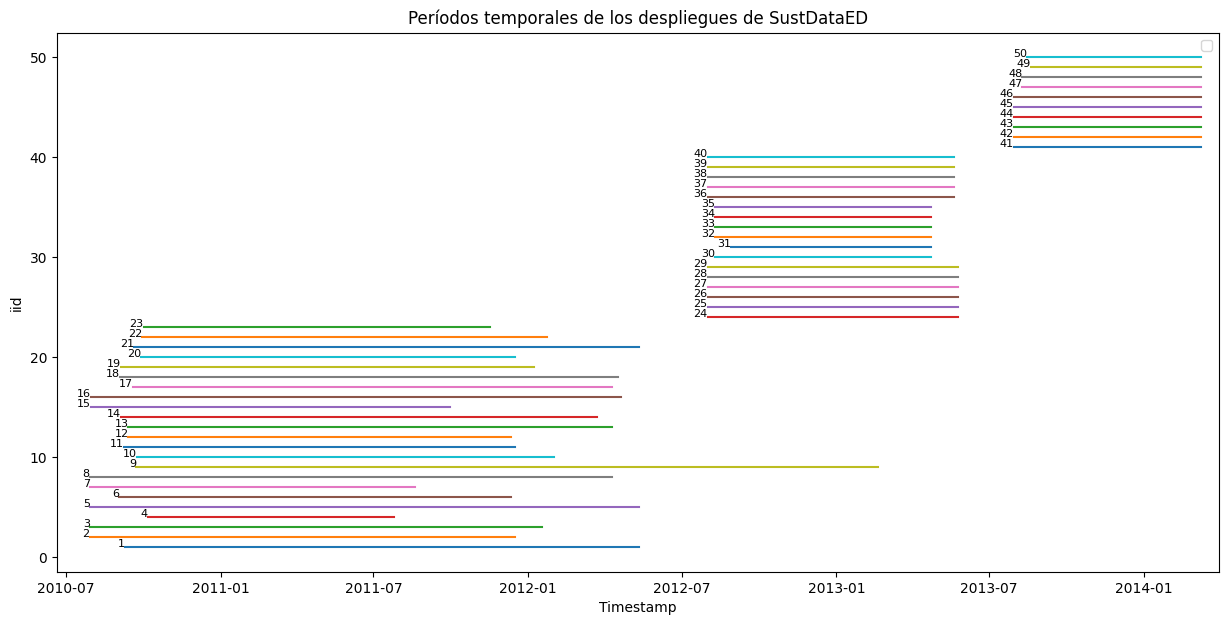
\includegraphics[width=1\textwidth,height=8.5cm]{img/diseno/despliegues.png}
    \caption{Representación del período temporal que comprende el proceso de recolección de datos para cada hogar}
    \label{fig:despliegues}
\end{figure}

\subsubsection{Medidas de consumo de energía}

En la Tabla \ref{tab:consumo} se listan los campos que han sido definidos para la recolección de medidas de consumo de cada uno de los hogares. El dataset asocia los parámetros eléctricos a dos identificadores: uno para describir la vivienda de la que se están recogiendo los datos, y otro, para el despliegue al que pertenece. 

\vspace{3mm}

Por otro lado, se almacena para cada medida una marca de tiempo con la fecha, hora, minuto y segundo en la que se ha recogido la información y se incluye el parámetro \textit{miss\_flag} para indicar si para un determinado instante temporal se han adquirido datos de forma incorrecta, suponiendo filas vacías en el dataset.

\clearpage

\begin{table}[h!]
    \centering
    \begin{tabular}{|c|c|c|}
    \hline
    \rowcolor[HTML]{AAAAAA} 
    \multicolumn{1}{|c|}{\cellcolor[HTML]{AAAAAA}Campo} & \multicolumn{1}{c|}{\cellcolor[HTML]{AAAAAA}Descripción} & Unidades \\ \hline
    \textit{home\_id} & Identificador de vivienda monitorizada & - \\ \hline
    \textit{timestamp} & Instante temporal de medida & datetime \\ \hline
    \textit{deploy} & Identificador del despliegue & - \\ \hline
    \textit{Imin} & Corriente mínima & A \\ \hline
    \textit{Imax} & Corriente máxima & A \\ \hline
    \textit{Iavg} & Corriente media & A \\ \hline
    \textit{Vmin} & Tensión mínima & V \\ \hline
    \textit{Vmax} & Tensión máxima & V \\ \hline
    \textit{Vavg} & Tensión media & V \\ \hline
    \textit{Pmin} & Potencia activa mínima & W \\ \hline
    \textit{Pmax} & Potencia activa máxima & W \\ \hline
    \textit{Pavg} & Potencia activa media & W \\ \hline
    \textit{Qmin} & Potencia reactiva mínima & VAR \\ \hline
    \textit{Qmax} & Potencia reactiva máxima & VAR \\ \hline
    \textit{Qavg} & Potencia reactiva media & VAR \\ \hline
    \textit{Smin} & Potencia aparente mínima & VA \\ \hline
    \textit{Smax} & Potencia aparente máxima & VA \\ \hline
    \textit{Savg} & Potencia aparente media & VA \\ \hline
    \textit{PFmin} & Factor de potencia mínimo & - \\ \hline
    \textit{PFmax} & Factor de potencia máximo & - \\ \hline
    \textit{PFavg} & Factor de potencia medio & - \\ \hline
    \textit{miss\_flag} & Flag de valores vacíos & - \\ \hline
    \end{tabular}
    \caption{Tabla de medidas de consumo energético \cite{sustdata}}
    \label{tab:consumo}
\end{table}

Los parámetros de tensión (V) y corriente (I) se muestrean continuamente a una frecuencia de 8KHz y las medidas de potencia activa (P), reactiva (Q) y aparente (S) se cuantifican a un ratio de 50 muestras por segundo a partir de las siguientes expresiones \cite{sustdata}:

\[ S = I_{\text{RMS}} \cdot V_{\text{RMS}} \]
\[ P = S \cdot \cos(\phi) \]
\[ Q = S \cdot \sin(\phi) \]

    Donde:
\begin{itemize}
    \renewcommand{\labelitemi}{}
    \item \( I_{\text{RMS}} \) es la corriente eficaz (RMS).
    \item \( V_{\text{RMS}} \) es el voltaje eficaz (RMS).
    \item \( \phi \) es el ángulo de fase entre la corriente y el voltaje instantáneos.
\end{itemize}

\vspace{3mm}

No obstante, como se habia introducido en el Apartado \ref{sec:sustdataed} y se había definido en la Tabla \ref{tab:datasets}, todas estas medidas, una vez son recogidas, se almacenan en el dataset a una resolución de una muestra por minuto. Se introduce también en la Tabla \ref{tab:consumo} el valor de factor de potencia (PF) para medir la eficiencia del uso de energía en un sistema eléctrico. Se cuantifica a partir de la razón entre la potencia activa (P) y la potencia aparente (S), siendo ideal un valor de 1. 

\subsubsection{Medidas de eventos de potencia}

La información sobre los eventos de potencia se extrae de las medidas en crudo de potencia activa que, como se ha expresado en el apartado anterior, se producen a una frecuencia de muestreo de 50Hz. La Tabla \ref{tab:eventos} se dedica al proceso de detección de dichos eventos o, en otros términos, de identificación de cambios en la carga total de una vivienda. Como se ha introducido en la Sección \ref{sec:sustdata}, estos datos serían de gran utilidad en el caso de requerirse el empleo de técnicas de \gls{nilm}.   

\vspace{3mm}

El proceso de recolección de las muestras tiene como base un método estadístico que calcula la probabilidad de que se produzca un cambio del valor de potencia media entre dos instantes. Para ello, el algoritmo trabaja con dos ventanas temporales: una de detección, que cuantifica la probabilidad del cambio en una muestra determinada y otra de búsqueda de los valores mínimos y máximos de potencia, que define las posiciones de los eventos en la señal de potencia agregada. En referencia a esto, viene definido un cambio mínimo de potencia real de 30 W.

\vspace{3mm}

\begin{table}[h!]
    \centering
    \begin{tabular}{|c|c|c|}
    \hline
    \rowcolor[HTML]{AAAAAA} 
    \multicolumn{1}{|c|}{\cellcolor[HTML]{AAAAAA}Campo} & \multicolumn{1}{c|}{\cellcolor[HTML]{AAAAAA}Descripción} & Unidades \\ \hline
    \textit{home\_id} & Identificador de vivienda monitorizada & - \\ \hline
    \textit{timestamp} & Instante temporal de medida & datetime \\ \hline
    \textit{deploy} & Identificador del despliegue & - \\ \hline
    \textit{delta\_P} & Cambio real de potencia activa & W \\ \hline
    \textit{delta\_Q} & Cambio real de potencia reactiva & VA \\ \hline
    \textit{trace\_P} & Traza real de potencia activa del evento & W \\ \hline
    \textit{trace\_Q} & Traza real de potencia reactiva del evento & VAR \\ \hline
    \end{tabular}
    \caption{Tabla de medidas de eventos de potencia \cite{sustdata}}
    \label{tab:eventos}
\end{table}

\clearpage

\subsubsection{Medidas de producción de energía}
\label{sec:prodsustdata}

El dataset \textit{SustDataED} recoge a nivel global los datos respectivos a la producción de electricidad en intervalos de 15 minutos. La energía generada se desagrega según su fuente de procedencia, dando protagonismo a las fuentes renovables. En la Tabla \ref{tab:prod} se indican los campos que han sido definidos para cuantificar las medidas.

\vspace{3mm}

\begin{table}[h!]
    \centering
    \begin{tabular}{|c|c|c|}
    \hline
    \rowcolor[HTML]{AAAAAA} 
    \multicolumn{1}{|c|}{\cellcolor[HTML]{AAAAAA}Campo} & \multicolumn{1}{c|}{\cellcolor[HTML]{AAAAAA}Descripción} & Unidades \\ \hline
    \textit{timestamp} & Instante temporal de medida & datetime \\ \hline
    \textit{total} & Producción total & MWh \\ \hline
    \textit{thermal\_fuel} & Electricidad producida por fuentes térmicas & MWh \\ \hline
    \textit{hydro} & Electricidad producida por fuentes hidroeléctricas & MWh \\ \hline
    \textit{eolic} & Electricidad producida por fuentes eólicas & MWh \\ \hline
    \textit{photovoltaic} & Electricidad producida por fuentes fotovoltaicas & MWh \\ \hline
    \end{tabular}
    \caption{Tabla de medidas de producción de energía \cite{sustdata}}
    \label{tab:prod}
\end{table}

\subsubsection{Medidas demográficas}

Para el análisis del comportamiento eléctrico de cada uno de los hogares monitorizados se puede visualizar en la Tabla \ref{tab:demo} cómo se almacena la información respectiva a sus inquilinos y a los períodos de adquisición de datos de cada vivienda.

\vspace{3mm}

\begin{table}[h!]
    \centering
    \begin{tabular}{|c|c|c|}
    \hline
    \rowcolor[HTML]{AAAAAA} 
    \multicolumn{1}{|c|}{\cellcolor[HTML]{AAAAAA}Campo} & \multicolumn{1}{c|}{\cellcolor[HTML]{AAAAAA}Descripción} & Unidades \\ \hline
    \textit{home\_id} & Identificador de vivienda monitorizada & - \\ \hline
    \textit{building\_id} & Identificador de edificio & - \\ \hline
    \textit{begin\_monitoring} & Fecha de inicio de medición & datetime \\ \hline
    \textit{end\_monitoring} & Fecha de fin de medición & datetime \\ \hline
    \textit{begin\_feedback} & Fecha de inicio de realimentación en el despliegue & datetime \\ \hline
    \textit{end\_feedback} & Fecha de fin de realimentación en el despliegue & datetime \\ \hline
    \textit{type} & Tipo de vivienda & - \\ \hline
    \textit{bedrooms} & Número de habitaciones & - \\ \hline
    \textit{adults} & Número de adultos inquilinos & - \\ \hline
    \textit{children} & Número de niños inquilinos & - \\ \hline
    \textit{contracted\_power} & Potencia contratada & kWh \\ \hline
    \end{tabular}
    \caption{Tabla de medidas de producción de energía \cite{sustdata}}
    \label{tab:demo}
\end{table}

De forma adicional, el dataset \textit{SustDataED} incluye otra tabla con datos complementarios sobre las personas participantes en los despliegues, como son el género, edad, educación y ocupación.

\subsubsection{Medidas de eventos de usuario}

Una de las ventajas que proporciona la monitorización del comportamiento eléctrico de un hogar es la realimentación de la información que se produce hacia los mismos usuarios. El dataset recoge en forma de eventos las interacciones que se llevan a cabo con este sistema de realimentación a través de los campos determinados en la Tabla \ref{tab:users}. 

\vspace{3mm}

\begin{table}[h!]
    \centering
    \begin{tabular}{|c|c|c|}
    \hline
    \rowcolor[HTML]{AAAAAA} 
    \multicolumn{1}{|c|}{\cellcolor[HTML]{AAAAAA}Campo} & \multicolumn{1}{c|}{\cellcolor[HTML]{AAAAAA}Descripción} & Unidades \\ \hline
    \textit{home\_id} & Identificador de vivienda monitorizada & - \\ \hline
    \textit{timestamp} & Instante temporal de medida & datetime \\ \hline
    \textit{deploy} & Identificador del despliegue & - \\ \hline
    \textit{type} & Tipo de interacción & - \\ \hline
    \textit{view\_id} & Identificador de pantalla de visualización & - \\ \hline
    \textit{view\_name} & Nombre de pantalla de visualización & - \\ \hline
    \end{tabular}
    \caption{Tabla de medidas de eventos de usuario \cite{sustdata}}
    \label{tab:users}
\end{table}

\subsubsection{Medidas de condiciones ambientales y climáticas}

Como se ha introducido al comienzo de la Sección \ref{sec:sustdataed}, el dataset aporta un enfoque medioambiental a los procesos de consumo y producción energética al incluir la recolección de los datos relativos a las condiciones climáticas que se dan en cada instante.

\vspace{3mm}

En la Tabla \ref{tab:env} se muestran los parámetros que se tienen en cuenta en las mediciones. Se incluye un campo dedicado a los eventos climáticos, que aporta información adicional cuando se produce un suceso metereológico determinado.

\vspace{3mm}

\begin{table}[h!]
    \centering
    \begin{tabular}{|c|c|c|}
    \hline
    \rowcolor[HTML]{AAAAAA} 
    \multicolumn{1}{|c|}{\cellcolor[HTML]{AAAAAA}Campo} & \multicolumn{1}{c|}{\cellcolor[HTML]{AAAAAA}Descripción} & Unidades \\ \hline
    \textit{timestamp} & Instante temporal de medida & datetime \\ \hline
    \textit{temperature} & Temperatura exterior & ºC \\ \hline
    \textit{humidity} & Humedad relativa & \% \\ \hline
    \textit{pressure} & Presión relativa & hPa \\ \hline
    \textit{wind\_dir} & Dirección del viento & - \\ \hline
    \textit{wind\_speed} & Velocidad del viento & kmh \\ \hline
    \textit{precipitation} & Niveles de precipitación & mm \\ \hline
    \textit{events} & Eventos relevantes & - \\ \hline
    \textit{conditions} & Condiciones del cielo & - \\ \hline
    \end{tabular}
    \caption{Tabla de medidas de condiciones ambientales \cite{sustdata}}
    \label{tab:env}
\end{table}

\subsection{Conclusiones del análisis del dataset \textit{SustDataED}}
\label{sec:conclusionessustdata}

Una vez realizado un estudio y un análisis en profundidad de los datos proporcionados por el dataset \textit{SustDataED}, se definen una serie de conclusiones a tener en cuenta antes de iniciar la fase de preprocesamiento de los datos. Por ello, considerando las motivaciones de la realización de este \gls{tfm}, se puede expresar que la utilidad que proporciona el dataset \textit{SustDataED} viene dada principalmente por el uso de las medidas de consumo, de producción y de las condiciones ambientales (ver Tablas \ref{tab:consumo}, \ref{tab:prod} y \ref{tab:env}). 

\vspace{3mm}

El procesamiento que será requerido para estos datos se detallará en la Sección \ref{sec:preprocesado}. No obstante, es importante destacar las características de los datos de producción eléctrica dados por \textit{SustDataED}. Como se ha expuesto anteriormente en la Sección \ref{prodsustdata}, el dataset proporciona esta información en términos globales y después, desagrega los valores energéticos según su fuente de procedencia. En la Sección \ref{sec:preprocesado} de este documento se detallará cómo será imprescindible determinar si estos datos son precisos y evaluar su utilidad específicamente en un entorno de \gls{sg}s como motivo de los objetivos de este \gls{tfm}.

\vspace{3mm}

Por otro lado, en cuanto a los eventos de potencia (ver Tabla \ref{tab:eventos}), como este \gls{tfm} no se basa en el diseño de técnicas \gls{nilm}, ni se pretende establecer una desagregación de potencia a nivel interno de una vivienda, se expone este tipo de datos únicamente a modo de estudio. De la misma forma, sucede en el caso de los eventos de usuario (ver Tabla \ref{tab:users}), los cuales no proporcionan información de utilidad que sea necesaria de procesar en la siguiente fase.

\section{Extracción de datos de producción}
\label{sec:global}

Como se ha expuesto en las conclusiones del dataset (ver Sección \ref{sec:conclusionessustdata}), en el siguiente paso de este \gls{tfm}, dedicado al preprocesamiento de los datos adquiridos (ver Sección \ref{sec:preprocesado}), se requerirá evaluar la precisión y la utilidad de los datos de producción proporcionados por \textit{SustDataED}. Para ello, esta Sección viene definida con el fin de obtener una fuente de datos de producción energética adicional, que permita contrastar la información adquirida del dataset anteriormente con la misma.

\vspace{3mm}

El proceso de simulación de los datos de producción energética implica recrear un dataset que sea riguroso con la realidad. Para ello, se debe realizar primero un estudio de las características de la localización para poder cuantificar los datos en función de la misma y de cada instante temporal. Posteriormente, se analizarán los resultados y se evaluará su precisión, con el fin de procesarlos y combinarlos con los datos adquiridos de \textit{SustDataED} (ver Sección \ref{sec:preprocesado}). Es decir, será en este paso de preprocesamiento donde se tome la decisión final de selección de la fuente de datos de producción más adecuada.

\subsection{Estudio y análisis de la ubicación}

En cuanto a la ubicación, en este caso será preciso basarse en Funchal, capital de la isla de Madeira (Portugal), ya que el análisis a realizar tiene que ser acorde a los datos recogidos en el dataset \textit{SustDataED}.

\vspace{3mm}

Según los parámetros de clasificación climática de Köppen \cite{koppen}, la ciudad de Funchal se caracteriza por tener un clima mediterráneo. Al ubicarse en una zona subtropical, presenta oscilaciones diarias mínimas, lo que se traduce en escasos cambios de temperatura entre las diferentes estaciones del año. Por ello, los inviernos son suaves y con precipitaciones moderadas, mientras que los veranos son ligeramente más cálidos y secos. 

\vspace{3mm}

No obstante, para el estudio de la generación energética mediante fuentes renovables, se va a poner el foco en el potencial de los recursos solares de la ubicación mediante el empleo del modelo solar denominado como \textit{Solargis}. Este modelo es proporcionado por la plataforma online \textit{Global Solar Atlas} \cite{globalsolar}, la cual es financiada por el \gls{esmap} y administrada por la organización de El Banco Mundial con el objetivo de mapear los recursos de energía renovable a nivel global. En otros términos, se permite el acceso a una gran cantidad mapas y de datos promediados a largo plazo de cualquier punto de la Tierra. \cite{energydata}

\vspace{3mm}

La información sobre los recursos solares y la cuantificación de la energía se suministran a través de esta plataforma siguiendo el estándar GIS ráster o cuadriculado con formatos GeoTIFF o AAIGRID. Para las diferentes capas de datos que se pueden determinar en función de los parámetros de radiación o del potencial fotovoltaico, se sigue una referencia espacial geográfica en base al código EPSG 4326 \cite{epsg}. Este código es asignado por la organización \gls{epsg} para identificar la proyección geográfica empleada, la cual en este caso hace referencia al sistema de coordenadas convencional (latitud-longitud) que se utiliza para la representación cartográfica de la Tierra. Por otro lado, los metadatos correspondientes a las características de cada capa se proveen en formato PDF o XML, siguiendo la estructura de datos geográficos definida por ISO 19115:2003/19139.~\cite{globalsolar} \cite{globalsolarreport}

\vspace{3mm}

Considerando las motivaciones que se persiguen con el empleo de la plataforma \textit{Global Solar Atlas}, es preciso realizar un paso previo al análisis, basado en la identificación de los tipos de capas de datos que se pueden configurar: \cite{globalsolarreport}

\begin{itemize}    
    \item \gls{dni} (kWh/m²): El índice de radiación directa normal se define como la cantidad de radiación solar que llega perpendicularmente a la superficie de la placa fotovoltaica, sin tener en cuenta los posibles efectos atmosféricos de dispersión o absorción.
    \item \gls{dif} (kWh/m²): El índice de radiación difusa hace referencia a la porción de radiación dispersada por los las nubes y los gases atmosféricos, lo que produce que provenga de todas las direcciones.
    \item \gls{ghi} (kWh/m²): El índice de radiación horizontal global viene dado por el sumatorio de la radiación solar directa (\gls{dni}) y la radiación solar difusa dispersada en consecuencia a los efectos de la atmósfera (\gls{dif}).
    \item \gls{gti} (kWh/m²): El índice de radiación global inclinada se refiere al total de radiación que incide en una superficie inclinada, que generalmente se encuentra ajustada un ángulo óptimo para maximizar la captación en términos anuales. 
    \item \gls{pvout} (kWh/kWp): El parámetro que mide el potencial energético de los sistemas fotovoltaicos de una ubicación determinada se cuantifica a partir de un sistema de referencia construido por módulos de silicio cristalino, de 1kWp y que se encuentra inclinado un ángulo óptimo.
\end{itemize}

Es necesario indicar que todos los parámetros anteriores se proporcionan para cada ubicación como valores promedios anuales de los totales diarios. Adicionalmente, otras capas a tener en cuenta para el análisis de los datos podrían ser la temperatura del aire, que determina en gran medida el ambiente de operación de las placas fotovoltaicas, o la elevación del terreno, que puede convertirse en un factor limitante para la instalación de plantas solares. 

\vspace{3mm}

En las Figuras \ref{fig:dni} y \ref{fig:ghi}, se visualizan en formato GeoTIFF los resultados de aplicar las capas de los índices de radiación \gls{dni} y \gls{ghi} al mapa mundial a través de la plataforma \textit{Global Solar Atlas}. Por otro lado, en la Figura \ref{fig:photo} se representa el potencial fotovoltaico dado por el parámetro \gls{pvout}. Como es de esperar, se puede verificar que existe una gran correlación entre los niveles de radiación que se recibe con respecto a la cantidad de energía que se puede generar con una planta solar en una ubicación determinada. 

\vspace{3mm}

\begin{figure}[H]
    \centering
    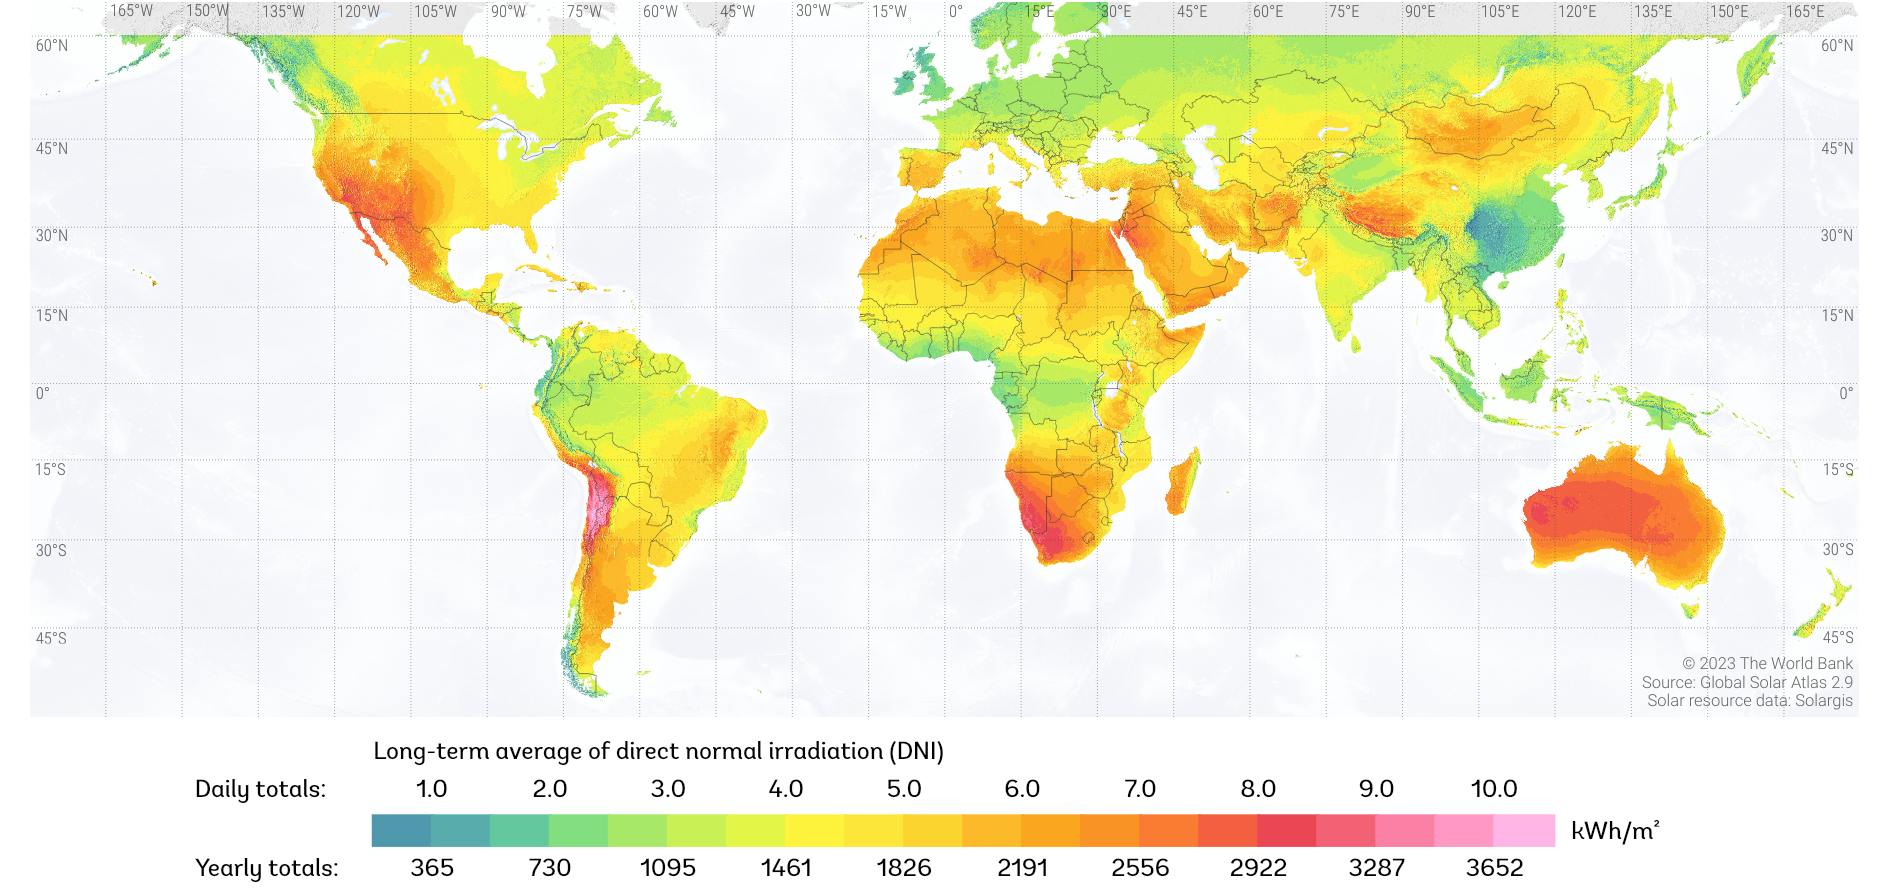
\includegraphics[width=1\textwidth]{img/diseno/dni.png}
    \caption{Mapa mundial del índice de radiación directa normal (\acrshort{dni}) mundial \cite{globalsolar}}
    \label{fig:dni}
\end{figure}

\begin{figure}[H]
    \centering
    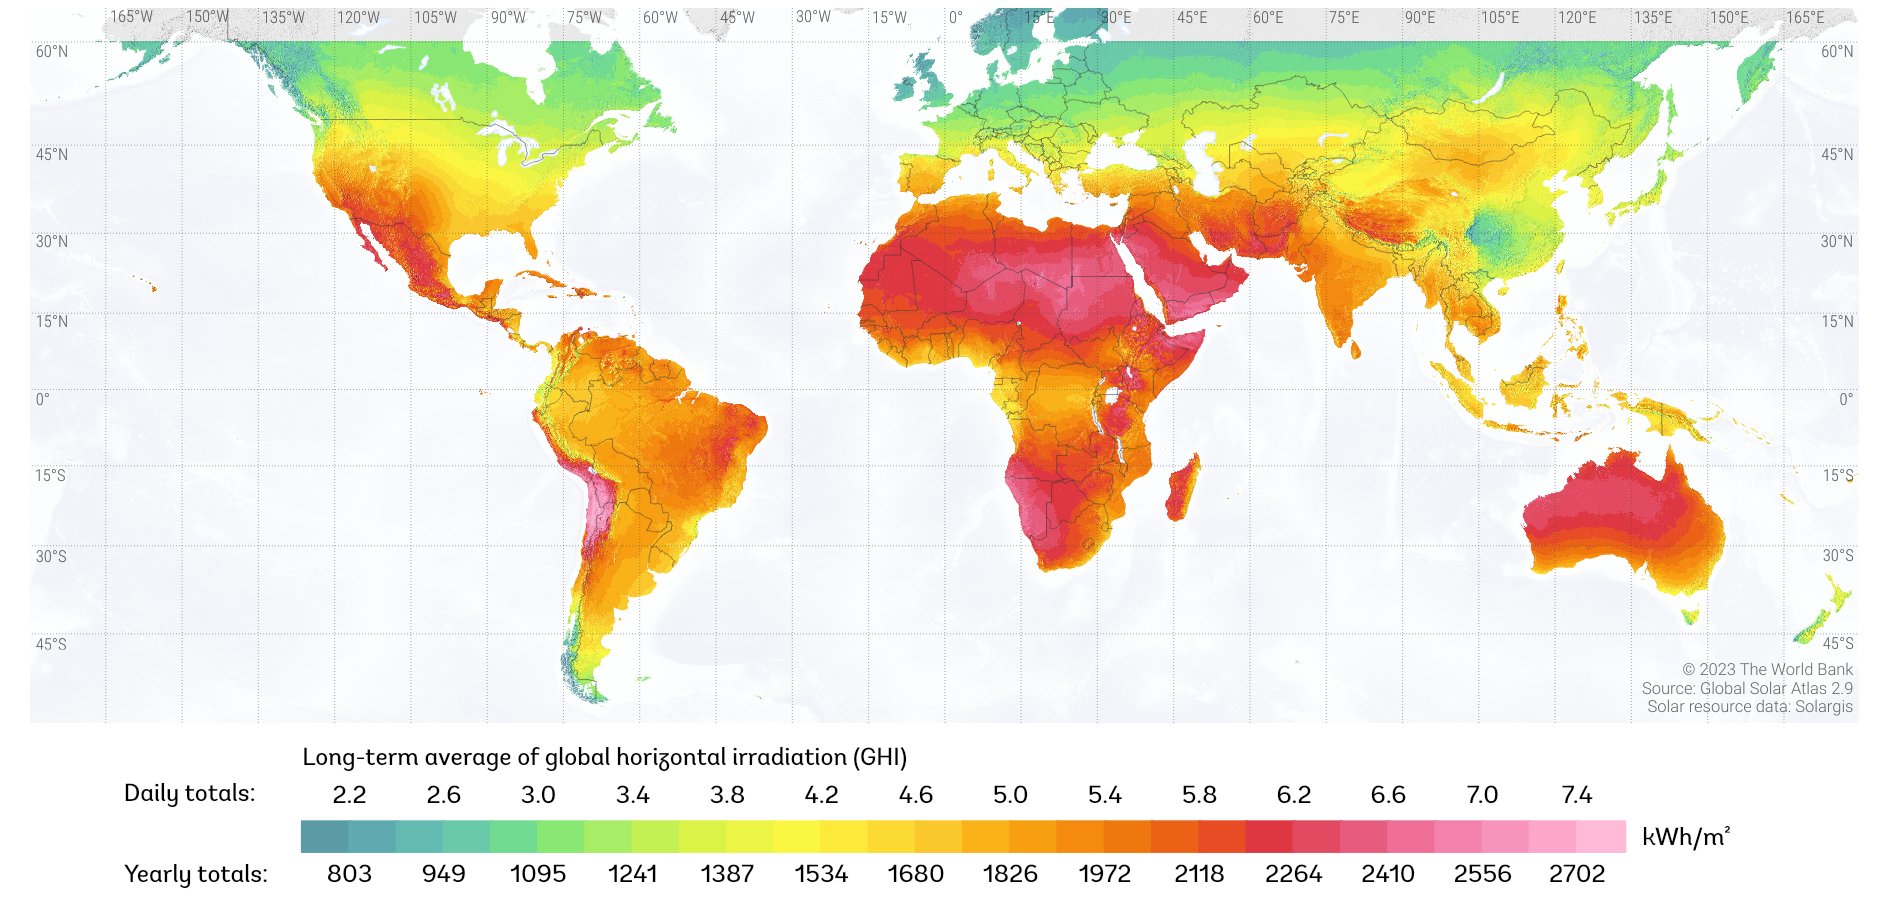
\includegraphics[width=1\textwidth]{img/diseno/ghi.png}
    \caption{Mapa del índice de radiación horizontal global (\acrshort{ghi}) mundial \cite{globalsolar}}
    \label{fig:ghi}
\end{figure}

\begin{figure}[H]
    \centering
    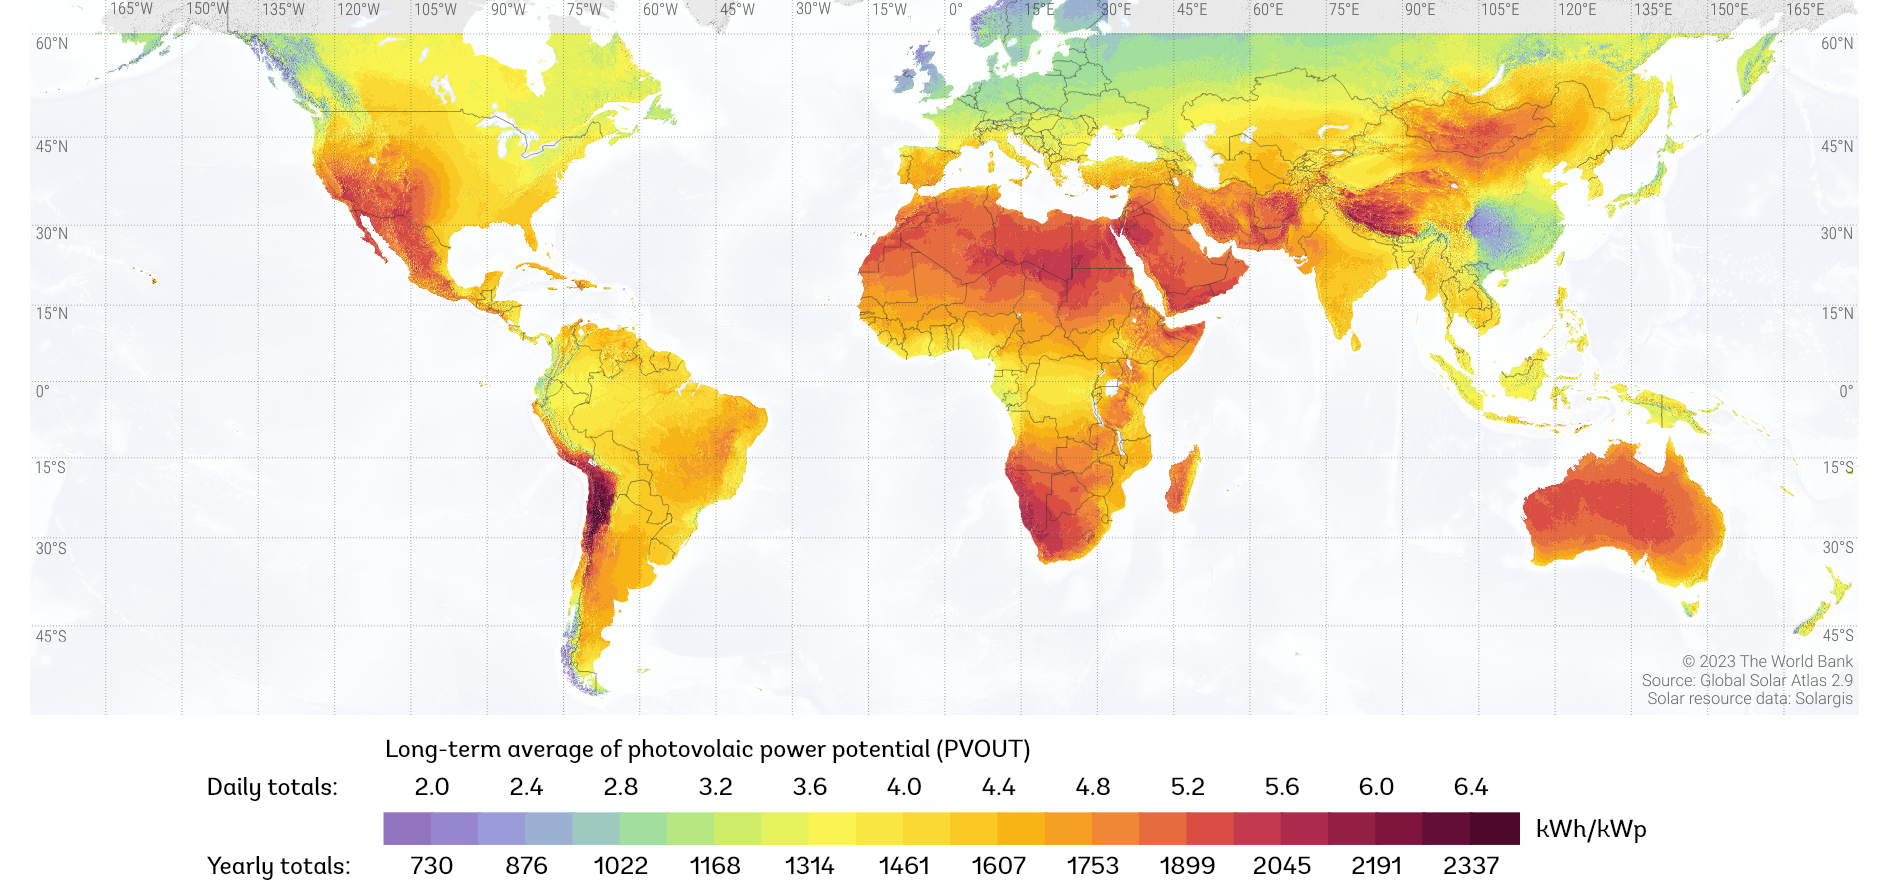
\includegraphics[width=1\textwidth]{img/diseno/photovoltaic.png}
    \caption{Mapa del potencial de producción energética fotovoltaica (\acrshort{pvout}) mundial \cite{globalsolar}}
    \label{fig:photo}
\end{figure}

\vspace{3mm}

En cuanto a la isla de Madeira, ocurre de la misma forma y se puede comprobar con más detalle a través de las Figuras \ref{fig:madeiradni}, \ref{fig:madeiraghi} y \ref{fig:madeirapvout}. Los valores para cada uno de los índices de radiación estudiados anteriormente se extraen específicamente desde la plataforma \textit{Global Solar Atlas} para el caso de la ciudad de Funchal y se recogen en la Tabla \ref{tab:global}.

\begin{table}[h!]
    \centering
    \begin{tabular}{|c|c|c|}
    \hline
    \rowcolor[HTML]{AAAAAA} 
    \multicolumn{1}{|c|}{\cellcolor[HTML]{AAAAAA}Parámetro} & \multicolumn{1}{c|}{\cellcolor[HTML]{AAAAAA}kWh/m²/día} & kWh/m²/año \\ \hline
    \gls{dni} & 3,698 & 1349,9 \\ \hline
    \gls{dif} & 2,038 & 743,8 \\ \hline
    \gls{ghi} & 4,345 & 1586,1 \\ \hline
    \gls{gti} & 4,730 & 1726,3 \\ \hline
    \end{tabular}
    \caption{Tabla de valores extraídos para cada índice de radiación en el municipio de Funchal~\cite{globalsolar}}
    \label{tab:global}
\end{table}





Para determinar el potencial energético que supondría la instalación de un sistema fotovoltaico, es preciso configurar los siguientes parámetros a través de la plataforma:





\begin{figure}[H]
    \centering
    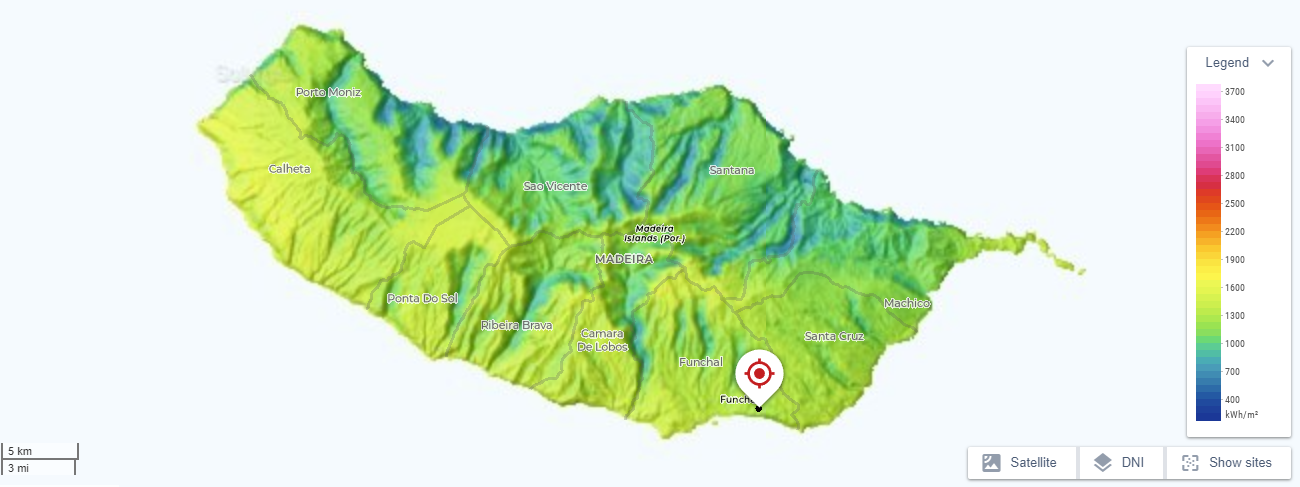
\includegraphics[width=1\textwidth]{img/diseno/madeiradni.png}
    \caption{Mapa del índice de radiación directa normal (\acrshort{dni}) de Madeira \cite{globalsolar}}
    \label{fig:madeiradni}
\end{figure}

\begin{figure}[H]
    \centering
    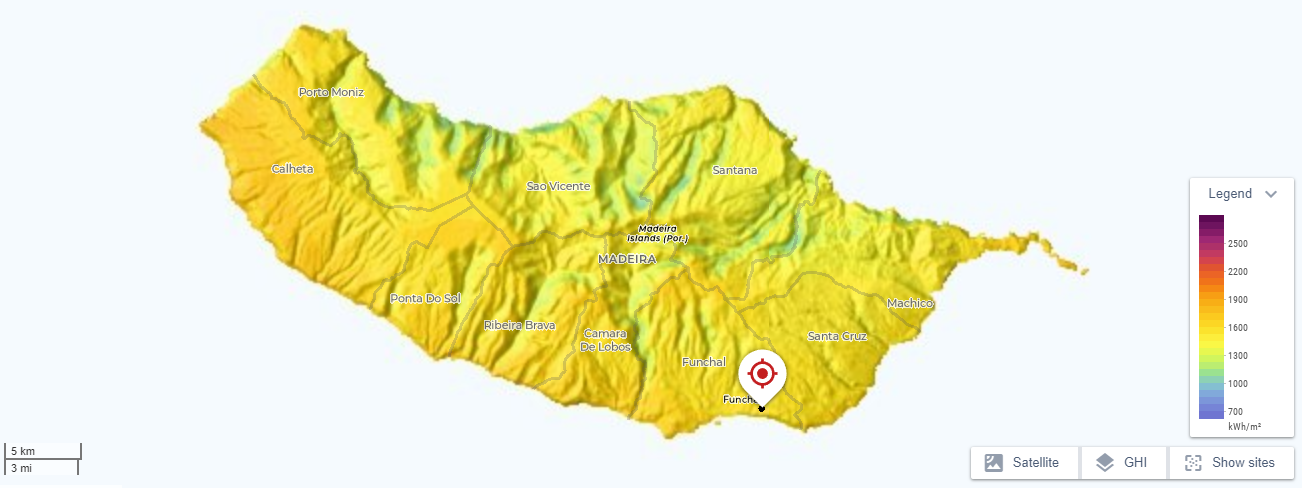
\includegraphics[width=1\textwidth]{img/diseno/madeiraghi.png}
    \caption{Mapa del índice de radiación horizontal global (\acrshort{ghi}) de Madeira \cite{globalsolar}}
    \label{fig:madeiraghi}
\end{figure}

\begin{figure}[H]
    \centering
    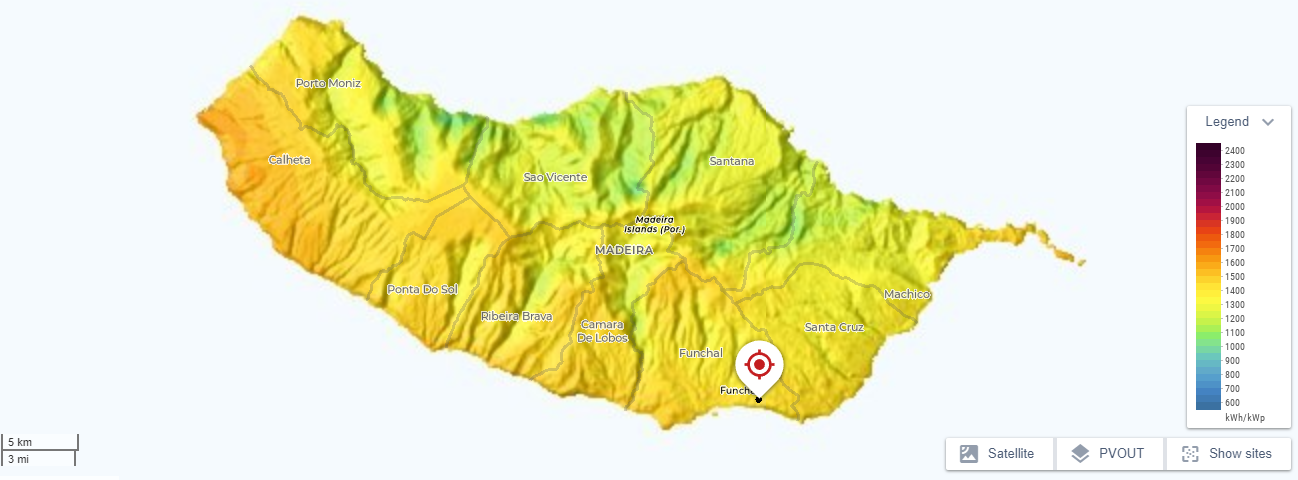
\includegraphics[width=1\textwidth]{img/diseno/madeirapvout.png}
    \caption{Mapa del potencial de producción energética fotovoltaica (\acrshort{pvout}) de Madeira \cite{globalsolar}}
    \label{fig:madeirapvout}
\end{figure}




% “En regiones con un buen recurso solar, como Madeira, un sistema solar residencial típico de tamaño moderado podría generar alrededor de 3 a 5 kilovatios-hora (kWh) por día por cada kilovatio pico (kWp) instalado.”




% •	Ver pdf PV Systems Performance in Madeira, gráficas interesantes, indica zonas de madeira con mayor producción
% •	Ver Solar Energy Resource in Madeira Islands, gráficas interesantes




 


\subsection{Extracción y cuantificación de los datos}

%Simulated solar data was generated by a tool provided by the US Department of Energy [4].

% •	HUE pdf -> Según bibliografía dataset HUE (este dataset solo tenía consumo residencial), la producción se calcula según ubicación y se elige Funchal, Madeira -> https://pvwatts.nrel.gov/pvwatts.php
